\chapter{Sistemi di Equazioni Non Lineari}

Fino ad ora siamo sempre stati abituati a problemi analitici dove la soluzione a un problema era data da un'equazione, o al più un piccolo sistema di equazioni non lineari. Tuttavia nella realtà sono molti i casi dove la soluzione viene trovata risolvendo complessi sistemi di equazioni non lineari, che non sempre possono essere svolti a mano. Da qui, la nascita di alcuni metodi di calcolo numerico che aiutano nella risoluzione di tali sistemi. Prima di illustrare questi metodi, ci soffermeremo brevemente su cos'è un'equazione non lineare:

\begin{definition}{Equazione non lineare}
    Un'\textbf{equazione non lineare} è un'equazione avente la forma
    \[ f(x) \eq 0 \]

    Chiamamo \textbf{soluzione} $\xi$ (o alternativamente \textbf{radici dell'equazione} o \textbf{zeri della funzione} $f$) di un'equazione non lineare quel valore tale che
    \[ f(\xi) \eq 0 \]
\end{definition}

All'interno di questo capitolo ci limiteremo prevalentemente al caso di radici reali. Per applicare un metodo su una funzione tuttavia, ci serve prima sapere le seguenti tre informazioni:
\begin{itemize}
    \item [1)] \textbf{quante} sono le radici (in questo caso, reali);
    \item [2)] \textbf{dove} si trovano, approssimativamente, le radici;
    \item [3)] se sono presenti delle \textbf{simmetrie} nella funzione.
\end{itemize}

Ci sono vari metodi per trovare queste informazioni: si può procedere allo \textbf{studio analitico}, alla \textbf{tabulazione} o all'analisi del \textbf{grafico} della funzione stessa. Procederemo ad illustrare tutti e tre i metodi su un'equazione di esempio:

\begin{example}
    Si consideri la seguente funzione $f(\lambda)$, che modella il tasso di crescita di una popolazione:
    \[ f(\lambda) \eq e^{\lambda} + \frac{0,435}{\lambda} (e^{\lambda} - 1) - 1,564 \eq 0 \]

    Procediamo a considerare lo \textbf{studio analitico} di questa funzione: notiamo che la funzione risulta definita e continua in $\mathbb{R} / \{0\}$, e studiando il semiasse positivo (non ha senso controllare il semiasse negativo, poiché quest'equazione modella la crescita della popolazione) notiamo che:
    \[ \lim_{\lambda \to 0} f(\lambda) < 0 \quad\quad \text{e} \quad\quad \lim_{\lambda \to +\infty} f(\lambda) \eq +\infty \]

    Calcolando la derivata prima, otteniamo invece la seguente funzione:
    \[ f'(\lambda) \eq e^{\lambda} + \left( 1 + 0,435 \frac{\lambda - 1}{\lambda^2} \right) + \frac{0,435}{\lambda^2} > 0 \]

    Notiamo infatti che il comportamento della funzione è positivo oltre lo 0: questo significa che la funzione $f(\lambda)$ è monotona crescente. Possiamo dunque concludere che, nel semiasse positivo, sia presente un unico zero $\xi$.
    \nwl
    Per il metodo della \textbf{tabulazione}, si considerano i valori ottenuti dalla funzione in corrispondenza di valori equidistanti di $\lambda$, e si osserva dunque il segno dei valori ottenuti. Ad esempio:
    \begin{center}
        \begin{tabular}{c|c}
            $\lambda$ & $f(\lambda)$ \\
            \hline
            $0,10$ & $-0,001335588295285$ \\
            $0,12$ & $0,025672938554613$ \\
            $0,14$ & $0,053195959592184$ \\
            $0,16$ & $0,081243551500795$ \\
            $0,18$ & $0,109825990666185$ \\
            $0,20$ & $0,138953757158539$ \\
        \end{tabular}
    \end{center}

    Come possiamo notare, abbiamo un cambio di segno tra $\lambda \eq 0,10$ e $\lambda \eq 0,12$: questo vuol dire che la radice della funzione si trova nell'intervallo $[0,10, \; 0,12]$. Possiamo anche osservare la radice usando un grafico della funzione:
    \begin{center}
        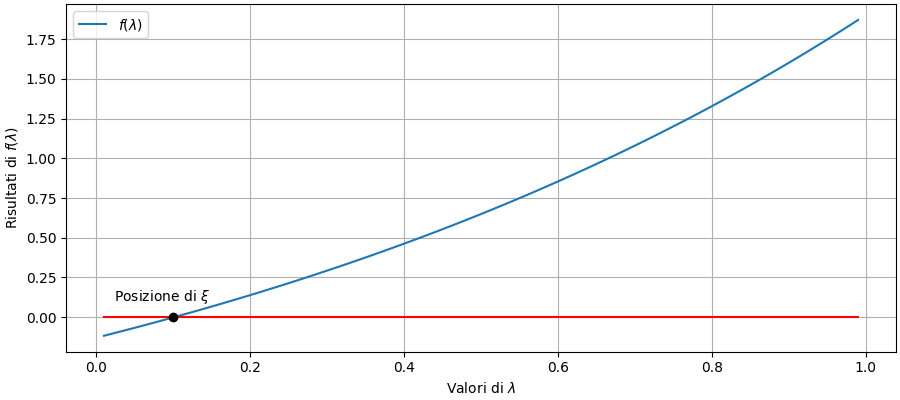
\includegraphics[width=\linewidth]{assets/image-002.png}
    \end{center}
\end{example}

Come abbiamo potuto notare dall'esempio, grazie ai tre metodi possiamo trovare una posizione approssimativa delle varie radici di una funzione. Ma come mai ci interessa tanto sapere la posizione di dove la funzione cambia segno? Perché grazie al \textbf{teorema di Bolzano}, questo ci permette di localizzare una radice.

\begin{theorem}{Teorema di Bolzano}
    Dato un \textbf{intervallo} $[a, \; b]$ e una \textbf{funzione} $f(x)$ \textbf{continua}, se $f(a)$ ha \textbf{segno discorde} rispetto a $f(b)$ (quindi, se $f(a) \cdot f(b) < 0$), allora $f(x)$ \textbf{interseca almeno una volta} l'asse delle $x$
\end{theorem}

È importante tuttavia sapere anche restringere l'intervallo di osservazione delle radici. Supponiamo di avere in esame la funzione
\[ p(x) \eq x^4 + 2x^3 + 7x^2 - 11 \eq 0 \]

mostriamo qui due grafici della funzione, in intervalli diversi:
\begin{center}
    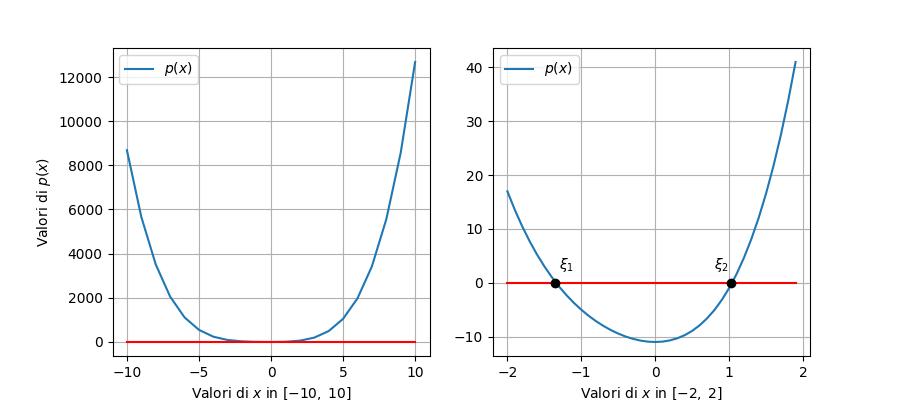
\includegraphics[width=\linewidth]{assets/image-003.png}
\end{center}

Notiamo come, in base all'intervallo, è più semplice notare la posizione delle radici. Infatti, $p(x)$ ha 4 radici, di cui due reali e due complesse coniugate.

\section{Metodo di Bisezione (o Dicotomico)}

Tra i vari metodi utilizzabili per trovare le radici in una funzione, il più semplice e immediato da utilizzare è il \textbf{metodo di bisezione}, o \textbf{metodo dicotomico}. Questo metodo permette, una volta individuato un intervallo di separazione in cui si trova una \textbf{singola radice}, di costruire una successione $\{ x_k \}$ di approssimazioni di $\xi$. Per applicare dunque questo metodo vanno rispettate due condizioni, dette \textbf{ipotesi di applicabilità}:
\begin{itemize}
    \item è stato individuato un intervallo $I \eq [a, \; b]$, all'interno del quale è presente \textbf{un'unica radice} $\xi$;
    \item la funzione $f$ in esame deve essere \textbf{continua in} $I$ (formalmente, $f \in C^0 [a, \; b]$, dove $C^0$ è l'insieme di funzioni continue);
    \item i due estremi $a$ e $b$ devono avere \textbf{segno discorde} (dunque $f(a) \cdot f(b) < 0$).
\end{itemize}

In sintesi, il teorema di Bolzano deve essere rispettato all'interno del nostro intervallo $I$; il metodo di bisezione infatti usa estensivamente il suddetto teorema. Passiamo dunque ad esaminare l'algoritmo del metodo di bisezione:

\begin{algorithm}[H]
    \caption{Metodo di bisezione (o dicotomico)}
    \KwIng{L'intervallo $[a, b]$, la funzione $f(x)$ e la tolleranza}
    $a \gets a_0, \; b \gets b_0$\;
    $\xi_{\text{seq}} \gets \{\}$ \tcp*{$\xi_{\text{seq}}$ è una sequenza vuota}
    \For{$k$ in $1, \; 2, \; 3, \; ...$}{
        $x_k \gets \frac{a + b}{2}$\;
        $d \gets |x_k - x_{k - 1}|$\;
        \BlankLine
        Add $x_k$ to $\xi_{\text{seq}}$\;
        \BlankLine
        \tcp{Se si trova la radice oppure viene raggiunta la tolleranza, l'algoritmo si ferma}
        \If{$(f(x_k) = 0)$ \textbf{or} $(d < \text{tol})$}{
            \textbf{return} $\xi_{\text{seq}}$
        }
        \BlankLine
        \tcp{In base all'intervallo che contiene la radice, ripetere l'algoritmo con l'intervallo aggiornato}
        \If{$f(a) \cdot f(x_k) < 0$}{
            $a \gets a, \; b \gets x_k$
        }
        \BlankLine
        \If{$f(x_k) \cdot f(b) < 0$}{
            $a \gets x_k, \; b \gets b$
        }
    }
\end{algorithm}

\nwl
Per il metodo di bisezione, l'idea è che dato un intervallo $I = [a, \; b]$, \textbf{dividendo} $I$ sempre \textbf{in sotto-intervalli} più contenuti, riusciremmo eventualmente ad ottenere un intervallo più piccolo all'interno del quale troveremmo la nostra radice $\xi$. Ogni sotto-intervallo è costituito da una delle due metà di $I$. Per sapere quale sotto-intervallo contiene $\xi$, basta applicare il teorema di Bolzano. L'algoritmo è semplice, e genera una successione di tutte le approssimazioni di $\xi$, denominata $\{x_k\}$ (o, nell'algoritmo, $\xi_{\text{seq}}$). La precisione del metodo di bisezione è ottenibile calcolando il relativo \textbf{errore di troncamento}.

\begin{definition}{Errore di troncamento}
    L'\textbf{errore di troncamento} è l'errore commesso \textbf{approssimando} la radice $\xi$ con il $k$-esimo elemento della successione creata tramite l'algoritmo del metodo di bisezione
    \[ e_k \eq \xi - x_k \]
\end{definition}

Ma l'algoritmo \textbf{può convergere}? Intuitivamente, convergerà verso $\xi$ solo se l'errore si dovesse ridurre a 0. Formalmente, possiamo esprimere questa relazione come
\[ \lim_{k \to \infty} x_k \eq \xi \quad \Longleftrightarrow \quad \lim_{k \to \infty} |e_k| \eq 0 \]

Possiamo però esprimere $e_k$ anche in altri termini. Per il metodo di bisezione, noi sappiamo che alla $k$-esima iterazione, $\xi$ sarà presente solo in $[a_{k - 1}, \; x_k]$ o in $[x_k, \; b_{k - 1}]$.

\begin{center}
    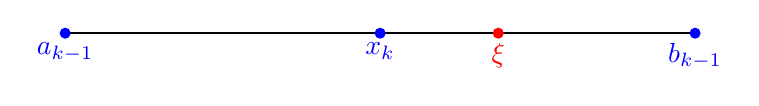
\begin{tikzpicture}
        \draw[black, thick] (0, 0) -- (8, 0);
        \fill[blue] (0, 0) circle (2pt) node [below] {$a_{k - 1}$};
        \fill[blue] (4, 0) circle (2pt) node [below] {$x_k$};
        \fill[blue] (8, 0) circle (2pt) node [below] {$b_{k - 1}$};
        \fill[red] (5.5, 0) circle (2pt) node [below] {$\xi$};
    \end{tikzpicture}
\end{center}

Dunque, data una generica iterazione $x_k$, l'errore di troncamento alla suddetta sarà uguale a
\[ |e_k| < \frac{b_{k - 1} - a_{k - 1}}{2} \]

Ora, siccome l'intervallo $[a_{k - 1}, \; b_{k - 1}]$ ha ampiezza pari alla metà dell'intervallo all'iterazione precedente (dunque $[a_{k - 2}, \; b_{k - 2}]$), possiamo costruire anche una formula generica dell'errore per qualsiasi iterazione $k$:
\[ |e_k| < \frac{b_{k - 1} - a_{k - 1}}{2} = \frac{b_{k - 2} - a_{k - 2}}{2^2} \eq \; ... \; \eq \frac{b - a}{2^k} \]

Dunque, anche il limite di prima può essere riscritto come
\[ 0 \leq \lim_{k \to \infty} |e_k| < \lim_{k \to \infty} \frac{b - a}{2^k} = 0 \]

\subsection{Ordine di corvengenza e Criteri di arresto}

Abbiamo visto che il metodo di bisezione converge, ma è anche importante che converga in tempi rapidi. Come possiamo determinare la "velocità" di convergenza? Questo viene determinato in base a un valore chiamato \textbf{ordine di convergenza} $p$.

\begin{definition}{Ordine e Fattore di Convergenza}
    Sia $\{ x_k \}$ una successione di approssimazioni \textbf{convergente} a $\xi$. Si dice che la successione ha un \textbf{ordine di convergenza} $p$ e un \textbf{fattore di convergenza} $C$ se esistono due numeri reali $p \geq 1$ e $C > 0$ tali che
    \[ \lim_{k \to \infty} \frac{|e_{k + 1}|}{|e_k|^p} \eq C \]

    Se $p \eq 1$, si dice che la convergenza è \textbf{lineare}, se $p \eq 2$, si dice invece che la convergenza è \textbf{quadratica}.
\end{definition}

Applicando la definizione di ordine e fattore di convergenza al metodo di bisezione, otteniamo che, per $k \to \infty$, si ha:
\[ \frac{|e_{k + 1}|}{|e_k|^p} \eq \frac{\frac{b - a}{2^{k + 1}}}{\frac{b - a}{2^k}} \eq \frac{2^k}{2^{k + 1}} \eq \frac{2^k}{2^k} \cdot \frac{1}{2} \eq \frac{1}{2} \]

Cosa ci dice il risultato appena ottenuto? Che, supponendo una convergenza lineare, otteniamo un fattore di convergenza di $\nicefrac{1}{2}$. Questo ci dice che la convergenza è in realtà \textbf{lenta}: ad ogni step dell'algoritmo riusciamo a dimezzare l'errore, e guadagnamo una cifra binaria per meglio esprimere il nostro risultato. Siccome $2^{-4} < 10^{-1} < 2^{-3}$, allora ogni 3 o 4 iterazioni si riesce a guadagnare una cifra decimale.
\nwl
Tuttavia, a causa degli errori di arrotondamento e troncamento da parte del computer, è praticamente impossibile che si riesca a raggiungere $f(x_k) \eq 0$. Dunque, quando dovremmo interrompere i calcoli? Possiamo definire dei \textbf{criteri di arresto a posteriori}, ovverosia
\[ \begin{cases}
|e_k| \simeq |x_k - x_{k - 1}| < \epsilon & \text{Se l'errore diventa minore di una tolleranza } \epsilon ... \\
|f(x_k)| < \epsilon & \text{...o se la funzione ritorna numeri minori della tolleranza } \epsilon
\end{cases} \]

Nel caso dell'algoritmo di bisezione, è stato scelto in precedenza di usare il primo criterio, ma potevano essere usati entrambi i criteri. Possiamo anche calcolare \textbf{a priori} una stima di quante iterazioni $K$ avremo bisogno prima di ottenere un errore minore di $\epsilon_{\text{min}}$. Per farlo, ci avvaliamo della formula dell'errore di troncamento:
\[ |e_k| < \frac{b - a}{2^k} < \epsilon_{\text{min}} \quad \Longrightarrow \quad K > \frac{\log(b - a) - \log(\epsilon_{\text{min}})}{\log(2)} \]

$K$ dovrà essere arrotondato all'intero più vicino, in quanto deve essere un intero positivo.